\begin{synthesecours}[Étude qualitative de fonctions]

\TitreSansTemps{Synthèse}
\end{synthesecours}


\begin{DefT}{Domaine de définition}
Soit $f$ une fonction. \\
Le domaine de définition de $f$ est l'ensemble des valeurs de la variable (souvent appelée $x$) qui admettent une image par $f$.
\end{DefT}


\begin{Rq}
Un intervalle est un ensemble de nombres. Les valeurs extrêmes de l'intervalle sont appelées \textbf{bornes de l'intervalle}. Le domaine de définition est donc un intervalle.
\end{Rq}


\begin{DefT}{Courbe}
Soit $f$ une fonction définie sur un intervalle I. \\
On appelle courbe de la fonction $f$, aussi appelée représentation graphique de $f$, l'ensemble des points $M$ du plan dont les coordonnées sont $(x,f(x))$, où $x$ parcourt le domaine de définition de $f$.
\end{DefT}

\begin{DefT}{Tableau de variations}\index{Tableau de variations}
Un tableau de variations d'une fonction $f$ est un tableau dans lequel l'étude synthétise
\begin{description}
\item[•] le domaine de définition de $f$ explicitement,
\item[•] les variations de $f$ à l'aide de flèches,
\item[•] les maximum et minimum.
\end{description} 

\begin{tikzpicture}
\tkzTabInit[lgt=2,espcl=3]{ $x$ / 1,$f$  / 2}
{ $0$ ,$3$,$5$}
\tkzTabVar{+/$3$,-/$1$,+/$2$ }
\end{tikzpicture}
\end{DefT}


\begin{Rq}
La courbe représentative d'une fonction $f$ et le tableau de variations de $f$ correspondent.
\end{Rq}


\begin{DefT}{Variations - Approche visuelle}
Dans un tableau de variations,
\begin{description}
\item[•] Une fonction croissante sur un intervalle est représentée par une flèche qui monte sur cet intervalle.
\item[•] Une fonction décroissante sur un intervalle est représentée par une flèche qui descend sur cet intervalle.
\end{description}
\end{DefT}



\begin{DefT}{Visualisation d'une fonction croissante ou décroissante}\index{Représentation graphique!Fonction croissante, décroissante}
\begin{description}[leftmargin=*]
\item[•] Lorsque, sur un intervalle $I$, la courbe représentative d'une fonction monte sans portion horizontale, on dit que la fonction est \textbf{strictement croissante sur $I$}. Si la courbe représentative possède une portion horizontale, on dit que la fonction est \textbf{croissante sur $I$}.
\item[•] Lorsque, sur un intervalle $I$, la courbe représentative d'une fonction descend sans portion horizontale, on dit que la fonction est \textbf{strictement décroissante sur $I$}. Si la courbe représentative possède une portion horizontale, on dit que la fonction est \textbf{décroissante sur $I$}.
\end{description}
\end{DefT}




\begin{DefT}{Maximum, minimum}
On dit que
\begin{description}[leftmargin=*]
\item[•] $M$ est le maximum de $f$ sur son domaine de définition si pour tout réel $x$ de $I$, $f(x) \leq M$. 
\item[•] $m$ est le minimum de $f$ sur son domaine de définition si pour tout réel $x$ de $I$, $f(x) \geq m$. 
\end{description} 
On dit que $f$ est bornée  sur $I$ lorsque $f$ accepte un maximum \textbf{et} un minimum sur $I$.
\end{DefT}


 

\begin{DefT}{Fonction croissante, décroissante sur $I$ - Approche comparatiste}
On dit que
\begin{description}[leftmargin=*]
\item[•] une fonction $f$ est \textbf{croissante sur $I$}, lorsque pour tout nombre $a$ et $b$ de $I$, les images de $a$ et de $b$ sont rangées dans le même ordre que $a$ et $b$.
\item[•] une fonction $f$ est \textbf{décroissante sur $I$}, lorsque pour tout nombre $a$ et $b$ de $I$,  les images de $a$ et de $b$ sont rangées dans l'ordre inverse de $a$ et $b$.
\end{description} 
\end{DefT}

 

\begin{DefT}{Fonction croissante, décroissante sur $I$  - Approche analytique }
\begin{description}[leftmargin=*]
\item[•] une fonction $f$ est \textbf{croissante sur $I$}, lorsque pour tout nombre $a$ et $b$ de $I$ tels que $a \leq b$, $f(a) \leq f(b)$.
\item[•] une fonction $f$ est \textbf{strictement croissante sur $I$}, lorsque pour tout nombre $a$ et $b$ de $I$ tels que $a \leq b$, $f(a) < f(b)$.
\item[•] une fonction $f$ est décroissante sur $I$, lorsque pour tout nombre $a$ et $b$ de $I$ tels que $a \leq b$, $f(a) \geq f(b)$.
\item[•] une fonction $f$ est décroissante sur $I$, lorsque pour tout nombre $a$ et $b$ de $I$ tels que $a \leq b$, $f(a) > f(b)$.
\end{description} 
\end{DefT}


